\input{./_path-to-root.ltx}
\documentclass[\PathToRoot/\ProjectName]{subfiles}
\whenstandalone{\externaldocument{\PathToRoot/\ProjectName}}

\begin{document}

\begin{figure}[htb] 
  \centering
  \caption{Wealth distribution fit by education group}
  \whenintegrated{\label{fig:LorenzPts}} 
  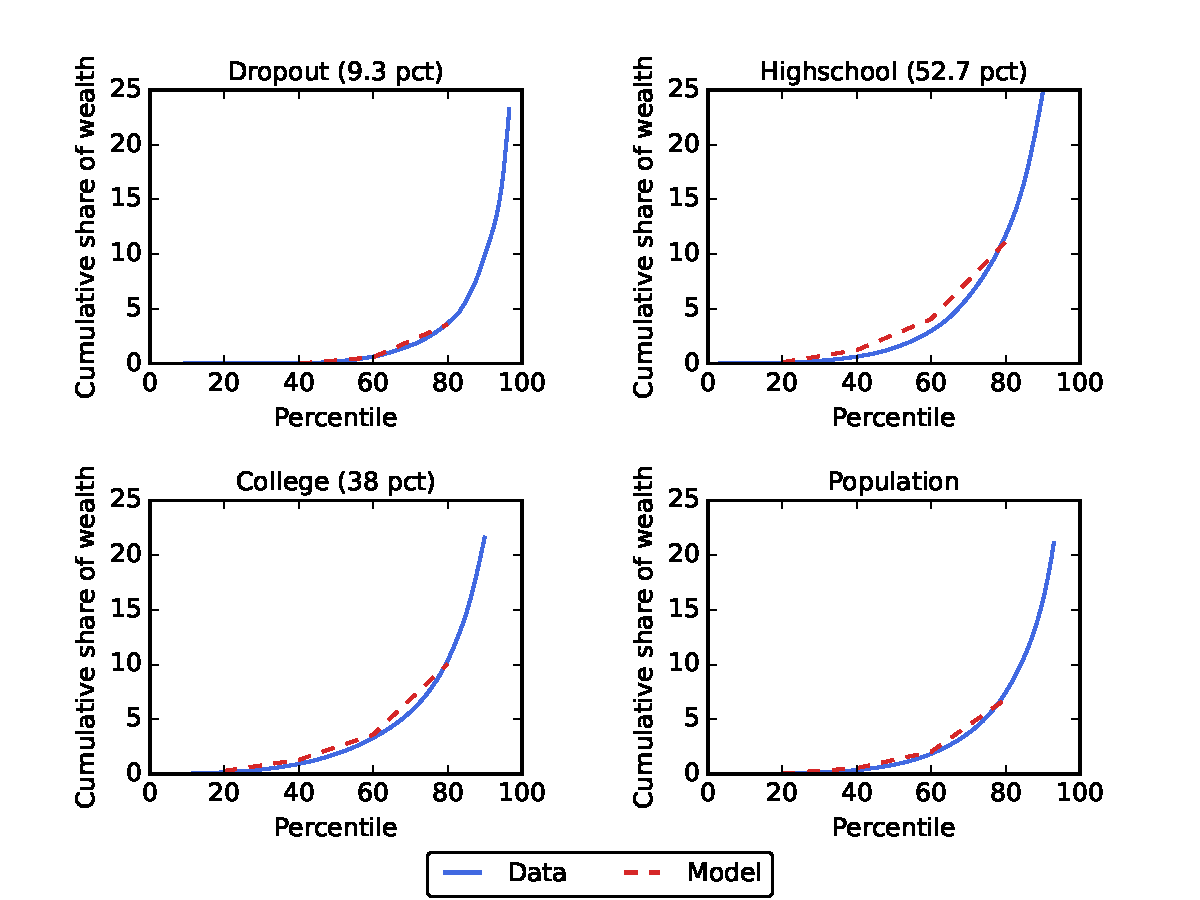
\includegraphics[width=.9\textwidth]{\PathToRoot/images/LorenzPoints_CRRA_2.0_R_1.01}

  \medskip
  \noindent\parbox{\textwidth}{\footnotesize
    \textbf{Note}: This figure validates the discount factor estimation methodology (Section~\ref{sec:estimBetas}).
    Separate discount factor distributions $\beta_e \pm \nabla_e$ are estimated for each education group
    to match the median liquid-wealth-to-permanent-income ratio and the 20th, 40th, 60th, and 80th
    percentile points of the Lorenz curve for liquid wealth.
    The model successfully avoids the ``missing middle'' problem identified by \cite{kaplanMPC2022},
    where insufficient wealth accumulation occurs in the middle of the distribution.
    The ``Population'' panel demonstrates that pooling the three calibrated education groups
    produces a realistic aggregate liquid wealth distribution.
  }
\end{figure}

\vspace{0.5em}

% Smart bibliography: Only include bibliography if standalone AND has citations
\smartbib

\end{document}
